\documentclass[12pt]{article}
\usepackage[a4paper, total={6.6in, 9in}]{geometry}

%\setlength{\parskip}{3pt}

\usepackage{amsmath}
\usepackage{amssymb}
\usepackage{bm}
\usepackage{graphicx}
\usepackage{siunitx}
\usepackage{authblk}
\usepackage{url}
\usepackage{appendix}
\usepackage{booktabs}
\usepackage[font=small]{caption}
\usepackage{subcaption}

\usepackage [english]{babel}
\usepackage [autostyle, english = american]{csquotes}
\MakeOuterQuote{"}

\bibliographystyle{ieeetr}

\begin{document}

\title{Can liquid crystal phases be identified via machine learning?}
\author{Joshua Heaton 10133722}
\affil{School of Physics and Astronomy, The University of Manchester}
\affil{MPhys project report}
\affil{Project performed in collaboration with James Harbon}
\date{\today}

\maketitle

\begin{abstract}
In this project, we investigate the application of machine learning models to the challenge of identifying liquid crystal phases directly from their texture images. Branching and sequential convolutional neural networks are applied to three distinct phase classification tasks, utilising training data in the form of liquid crystal texture images extracted from polarised microscopy videos. We obtain high mean test set accuracies, often greater than 90 percent, for sequential models classifying the isotropic, nematic, cholesteric, and smectic phases. Sequential and branching models perform very well in the binary classification of the smectic A and smectic C phases, with all models achieving a mean test set accuracy of above 90 percent. Models are also applied to the classification of the fluid smectic, hexatic smectic, and soft crystal phases. Success in this task is limited so far due to a lack of data for the hexatic smectic and soft crystal phases.
\end{abstract}

\pagenumbering{gobble}
\newpage
\tableofcontents

\pagenumbering{gobble}
\newpage
\pagenumbering{arabic}

%=========================================================================================
\section{Introduction}
Machine learning methods have seen widespread utilisation across all scientific disciplines, in situations where conventional algorithms are too cumbersome to implement for specific data-based and modelling tasks \cite{Carleo19}. Deep learning, loosely defined as machine learning with large datasets, parallel computation, and scalable algorithms with many layers \cite{Goodfellow16}, has and continues to increase the range and complexity of possible applications of machine learning in the sciences \cite{Carleo19}. Any task applying deep learning to data with a grid-like form, such as images, likely involves the usage of convolutional neural network (CNN) algorithms \cite{Goodfellow16}. CNNs were conceived in 1989 by Yann LeCun \textit{et al.} and successfully applied to the recognition of handwritten characters \cite{LeCun89}. However, their astounding performance in the field of computer vision would not be fully realised until after breakthroughs in deep learning, starting in 2006 \cite{Goodfellow16}. Their efficacy was further proven when Geoffrey Hinton \textit{et al.} entered a CNN into the ImageNet Large Scale Visual Recognition Challenge (ILSVRC) in 2012 and won by a large margin \cite{ILSVRC15}.

Liquid crystal phases are in general identified by eye, directly from textures taken by polarised microscopy. Without adequate experience, this can prove a difficult task. Certain unique liquid crystal phases, often generated by minor changes in structural properties, can have similar textural appearances \cite{Dierking03}. Our project aims to test the viability of machine learning algorithms as tools to assist phase identification. CNNs are particularly suitable due to their prevalence in image classification and form the core of our investigations. Current literature on this specific topic is limited, and the approaches so far have mostly involved the usage of simulated textures in the training of models \cite{Sigaki20, Minor20}. Sigaki et al. have demonstrated the viability of CNNs in isotropic and nematic phase texture classification and the prediction of physical liquid crystal properties \cite{Sigaki20}. Our study further explores and attempts to push the classification task limits across a wider range of phases, utilising real experimental data produced by polarised microscopy.

This project report will first provide a brief overview of the physics behind liquid crystals and the capturing of their textures by polarised microscopy, as well as an introduction to machine learning, neural networks, and CNNs. The details and results of our investigations into phase classification will then be presented, as well as an outlook to further study.
%=========================================================================================
\section{Background theory}
\subsection{Liquid crystal phases}
\subsubsection{Structure}
Liquid crystals are substances in a state between a fully isotropic liquid and a crystal with a periodic lattice structure \cite{Demus99, Dierking03}. The molecules can have varying positional order and have orientational order over large sections. The unit vector parallel to the alignment of the molecules is called the director \cite{Demus99, Dierking03}. Other details, such as molecular shape and chirality, affect the overall structure. These structural variations result in numerous individual identifiable liquid crystal phases \cite{Demus99, Dierking03}. Thermotropic liquid crystals exhibit phase transitions with changing temperature, whereas lyotropic liquid crystals are dissolved in a solvent with the phase depending on the concentration \cite{Demus99}. This project will be concerned with only thermotropic liquid crystals. 

When cooling a thermotropic liquid crystal, starting in the isotropic liquid (Iso) phase, it will first transition to the nematic (N) phase, which has orientational order only. If the chemical is chiral, the chiral nematic or cholesteric (N*) phase will, instead, be present. It also has no positional order and has a periodic variation of the director, resulting in helical structures. Upon further cooling, the smectic (Sm) phase is reached. This can be split into three categories, going from fluid smectic (FSm) to hexatic smectic (HSm) to soft crystal (SC) in order of decreasing temperature. The fluid smectic phase has molecules arranged in layers, with no positional order in the plane of each layer. When the director is perpendicular to the layer planes, the phase is smectic A (SmA), with smectic C (SmC) having a director that is tilted by comparison. Hexatic smectic phases have short-range positional order within the layer planes, with hexagonal intermolecular arrangements interspersed with order-breaking defects. This encompasses the smectic B (SmB), I (SmI), and F (SmF) phases. Smectic B has a director perpendicular to the layer planes, whereas for smectic I it is tilted towards the vertices of the hexagons, and towards the sides of the hexagons for smectic F. The soft crystal phases are defect-free within the layers and, therefore, exhibit long-range positional order \cite{Dierking03}.
\subsubsection{Polarised microscopy}
The liquid crystal texture data used in this project have been obtained by polarised microscopy captured with a video camera. In brief terms, a polarising microscope works by placing a sample between perpendicularly aligned polarisers. When unpolarised light is shone through the arrangement, the resulting image will be dark unless the sample rotates the plane of polarisation \cite{Dierking03}. For liquid crystals, the isotropic liquid phase has no optical properties and produces completely dark textures. The nematic, cholesteric and smectic phases are anisotropic and, therefore, birefringent, with optical axes depending on their structures. This produces unique textural image features for each phase \cite{Dierking03}. Some example textures taken from our dataset are displayed in Figure 1.

\begin{figure}[!htb]
\centering
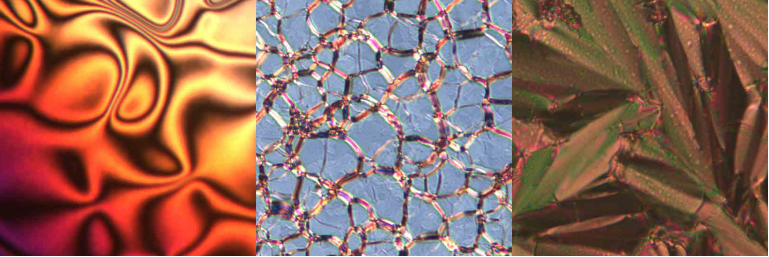
\includegraphics[width=6in]{images/texture_samples.png}
\caption{Liquid crystal textures from the dataset, from left to right: nematic phase compound 5CB, cholesteric phase compound D5, and smectic C phase compound M10.}
\end{figure}
%=========================================================================================
\subsection{General machine learning principles}
A machine learning model is a computer algorithm that automatically improves its performance in a given task as it gains experience from a dataset \cite{Goodfellow16}. It learns patterns in data and uses these patterns to make probabilistic predictions. The data normally takes the form of a set of $N$ examples, which are usually expressed as vectors, or some other structure of features, $\{\bm{x}^{(i)}\}_{i=1}^N$, containing quantitative information about example $i$ \cite{Murphy12}. In supervised learning the examples are given labels $y^{(i)}$, to form a training set of pairs $\{\bm{x}^{(i)}, y^{(i)}\}_{i=1}^N$, and the model attempts to learn the mapping from a general input $\bm{x}$ to an output $\hat{y}$. One main type of supervised learning is regression, in which the output is a numerical scalar. The other main type is classification, in which the model predicts what the input belongs to out of a selection of classes. Unsupervised learning does not use labels. The algorithm attempts to learn specific patterns in the dataset, such as clusters of similar data points \cite{Murphy12}. The topic of this project is a supervised classification problem.

A supervised model can usually be expressed as a function of inputs and a set of parameters $\bm\theta$ such that $\hat{y}=f(\bm{x};\bm\theta)$. The parameters are optimised by minimising a cost function $J(\bm\theta)$, which measures the deviation of model predictions from the true labels. The most common optimisation algorithms involve computing the gradient of $J(\bm\theta)$ with respect to $\bm\theta$ \cite{Goodfellow16}. 

The capacity of a model is akin to its complexity. The number of trainable parameters can give a fast indication of capacity. However, it also depends on the model's functional form. The parameters controlling model capacity and certain training settings are known as hyperparameters \cite{Goodfellow16}. If the capacity is too small, the model will tend to "underfit" the training set, resulting in poor performance even when optimised well. On the other hand, too high a capacity will result in "overfitting" with high performance on the training set. However, the model may have a high generalisation error, which is the error rate when evaluating it on new, unseen data \cite{Murphy12, Goodfellow16}. Before training begins, the entire dataset is often split into training, validation, and test sets, containing $N_{\mathrm{train}}$, $N_{\mathrm{valid}}$, and $N_{\mathrm{test}}$ examples respectively. The training set, as defined previously, is used to optimise the parameters. The model's performance is then evaluated on the validation set. Poor performance on both the training and validation sets indicates underfitting, whereas a high performance on the training set and low on the validation set suggests overfitting. The validation set can, therefore, be used to tune the hyperparameters of the model before retraining. This is repeated until the model fits optimally \cite{Murphy12, Goodfellow16}. The final model is evaluated on the unseen test set, providing an estimation of its generalisation error \cite{Murphy12}. Methods used to reduce generalisation error, such as reducing model capacity, are known as regularisation. \cite{Goodfellow16}.

Data leakage, with supervised learning, is when there are examples in the validation or test sets with a high degree of similarity to those in the training set. The model will easily produce the correct output when evaluated on the leaked examples, especially when overfitting occurs. This can result in a false indication of low generalisation error. Therefore, data leakage must be avoided to produce a reliable model \cite{Kaufman12}.
%=========================================================================================
\subsection{Feedforward neural networks}
\subsubsection{Forward propagation}
A neural network is a type of machine learning model that takes inspiration from the current understanding of how the brain works \cite{Minsky69}. The inputs are forward propagated through a series of connected hidden units, akin to neurons in a brain, before reaching the output units. In the simple case of a fully connected neural network, the units are arranged into layers, with each unit in a layer connected to every unit of the previous layer \cite{Rumelhart86}. We will define the total number of layers, excluding the input layer, as the depth, $D$, of the model, with the width, $W_l$, of layer $l\in[0..D]$ equal to the number of units it contains. $l=0$ is the input layer. The choice of hyperparameters $D$ and $W_l$ defines the architecture of the model \cite{Haykin98}. A schematic of an example network is presented in Figure 2. 

\begin{figure}[!htb]
\centering
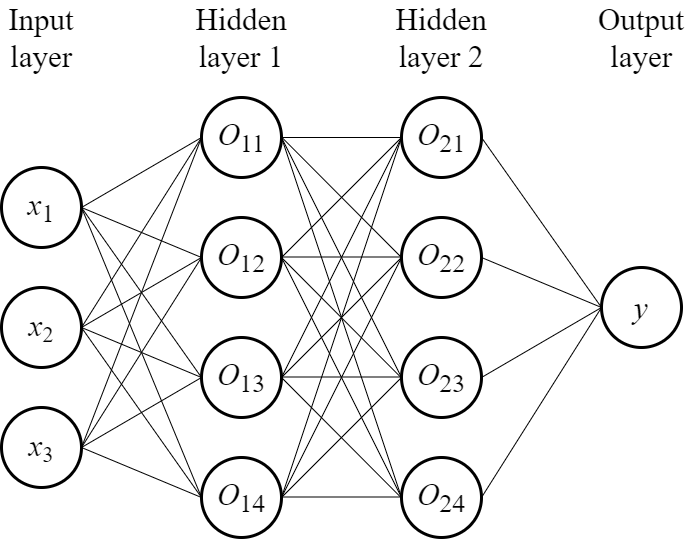
\includegraphics[width=3.5in]{images/feedforward_nn.png}
\caption{Diagram of a feedforward fully-connected neural network with three input values, $D=3$, $W_1=W_2=4$, and one output unit.}
\end{figure}

A single hidden unit's output value is calculated by multiplying the output of each of the previous layer's units with a weight parameter, summing these together with a bias parameter, and then passing the result through a non-linear activation function \cite{Rumelhart86}. More formally, the output $O_{lu}$ of hidden unit $u\in[1..W_l]$, of layer $l$, with bias parameter $b_{lu}$ and activation function $A(h)$, is calculated as
\begin{equation}
O_{lu}=A(h_{lu})
\end{equation}
with
\begin{equation}
h_{lu}=b_{lu}+\sum_{v=1}^{W_{l-1}}w_{luv}O_{(l-1)v}
\end{equation}
for $l > 0$. $w_{luv}$ is the weight parameter that hidden unit $u$ of layer $l$ applies to the output of unit $v\in[1..W_{l-1}]$ of the previous layer \cite{Haykin98}. $O_{0u}$ is equivalent to value $x_u$ of the input vector $\bm{x}$. In matrix form,
\begin{equation}
\bm{O}_l=A(\bm{h}_l)
\end{equation}
with
\begin{equation}
\bm{h}_l=\bm{w}_l\bm{O}_{l-1}+\bm{b}_l
\end{equation}
where $\bm{w}_l$ is the $W_l \times W_{l-1}$ dimensional matrix of weights for layer $l$, with rows corresponding to the weights of each hidden unit, $\bm{O}_l$ is the vector of outputs for layer $l$, and $\bm{b}_l$ is the vector of bias parameters for layer $l$. For the first hidden layer,
\begin{equation}
\bm{h}_1=\bm{w}_1\bm{x}+\bm{b}_1\; \cite{Haykin98}.
\end{equation}
The activation function is applied element-wise. A highly effective choice of activation function for hidden units, performing a similar operation to biological neurons, is the rectified linear unit (ReLU),
\begin{equation}
A(h)=\mathrm{max}(0,h)\; \cite{Glorot11}.
\end{equation}

The number of units in the final output layer depends on the type of model. For regression, there will be one unit that outputs a continuous-valued prediction \cite{Goodfellow16}. For classification, the number of final layer units is equal to the number of classes, $C=W_D$, with each one outputting the predicted probability that an input $\bm{x}$ belongs to a particular class. The network is therefore summarised as $\hat{\bm{y}}=f(\bm{x};\bm\theta)$, with $\hat{\bm{y}}$ being the $C$ dimensional vector of output probabilities and $\bm\theta$ the combined representation of all $\bm{w}_l$ and $\bm{b}_l$. Each example in the dataset is labelled by a vector $\bm{y}$, with a value of one for the component corresponding to the true class and zero for all other components. The component $y_u$, with $u\in[1..C]$, is equivalent to the Kronecker delta $\delta_{ut}$ where the index $t$ corresponds to the true class \cite{Goodfellow16}. The most common choice of final layer activation function for classification is the softmax function, $\sigma_{SM}(h)$, for which the components $\hat{y}_u$ of the output probability prediction vector are given by
\begin{equation}
\hat{y}_u=O_{Du}=\frac{e^{h_{Du}}}{\sum_{v=1}^{C}e^{h_{Dv}}}\;\cite{Goodfellow16}.
\end{equation} 
When there are just two classes, known as binary classification, only one unit is needed in the output layer. The data labels $y$ are equal to one or zero, depending on the class that $\bm{x}$ belongs to \cite{Goodfellow16}. The activation function in this case is generally the logistic sigmoid function, $\sigma(h)$, with
\begin{equation}
\hat{y}=O_D=\frac{1}{1+e^{-h_D}}.
\end{equation}
The value of $\hat{y}$ is the predicted probability that $\bm{x}$ belongs to one of the classes, with a probability of $1-\hat{y}$ that it belongs to the other \cite{Goodfellow16}. 

In 1989 Kurt Hornik \textit{et al.} mathematically proved that feedforward neural networks with multiple layers and non-linear activations can approximate any continuous function given the correct configuration \cite{Hornik89}. Another advantage of neural networks is that they can automatically learn to extract useful higher-level features from the raw input data \cite{Haykin98}.

\subsubsection{Training}
Neural network training starts with random initialisation of the weights, for example, by drawing values from a normal distribution \cite{Goodfellow16}. A single update step is generally carried out by calculating the model output for each example, followed by the gradient of the cost function with respect to the model weight parameters, $\bm{g}=\bm\nabla_{\bm\theta}J(\bm\theta)$. An iterative optimisation algorithm then uses the gradient to update the parameters to reduce the cost \cite{Goodfellow16}. $\bm{g}$ is obtained using the backpropagation algorithm, which calculates the gradient of $J(\bm\theta)$ with respect to the final outputs, and then recursively applies the chain rule going backwards through the network, calculating the derivatives with respect to the outputs of each hidden unit followed by their parameters \cite{Haykin98}. Backpropagation for neural networks is detailed in Appendix A.1. The overall goal of training iterations is to reduce the generalisation error of the model \cite{Goodfellow16}. Generally, the cost function is the expectation value of the loss of all examples in the training set,
\begin{equation}
J(\bm\theta)=\frac{1}{N_{\mathrm{train}}}\sum_{i=1}^{N_{\mathrm{train}}}L(f(\bm{x}^{(i)};\bm\theta),\bm{y}^{(i)})
\end{equation}
where the loss is the cross-entropy between the model's output probabilities and the input's true class label,
\begin{equation}
L(f(\bm{x};\bm\theta),\bm{y})=L(\hat{\bm{y}},\bm{y})=-\sum_{u=1}^Cy_u\mathrm{log}(\hat{y}_u)\; \cite{Goodfellow16}.
\end{equation}
When training a classifier model, the softmax activation function of the final layer can be combined with the loss function to give the categorical cross-entropy,
\begin{equation}
L_{CCE}(\hat{\bm{y}},\bm{y})=-\sum_{u=1}^Cy_u\mathrm{log}\,\sigma_{SM}(h_{Du})=-\mathrm{log}\left(\frac{e^{h_{Dt}}}{\sum_{j=1}^{C}e^{h_{Dj}}}\right)
\end{equation}
where we have used the fact that $y_u=\delta_{ut}$ for classification \cite{Kline05}. For binary classification in which the logistic sigmoid activation function is used, the binary cross-entropy is
\begin{equation}
L_{BCE}(\hat{y},y)=
\left\{
\begin{array}{ll}
-\mathrm{log}\,\sigma(h_D) & \mbox{if } y^{(\mathrm{true})}=1 \\
-\mathrm{log}\left(1-\sigma(h_D)\right) & \mbox{if } y^{(\mathrm{true})}=0
\end{array}
\right.\;\cite{Richard91}.
\end{equation}

Calculating the exact derivative of the cost function is extremely computationally expensive in most situations when $N_{\mathrm{train}}$ is large. Instead, an approximation of the gradient, $\hat{\bm{g}}$, is calculated by randomly sampling a "minibatch" of $m$ examples from the training data, giving
\begin{equation}
\hat{\bm{g}}=\frac{1}{m}\bm\nabla_{\bm\theta}\sum_{i=1}^mL(f(\bm{x}^{(i)};\bm\theta),\bm{y}^{(i)})\;\cite{Goodfellow16}.
\end{equation}
In general, the loss of precision from the difference between $\hat{\bm{g}}$ and the exact gradient $\bm{g}$ is outweighed by the greatly decreased training step computation time \cite{Goodfellow16}. Optimisation methods that use this random minibatch sampling are known as stochastic methods. Typically, a single parameter update step is performed on each minibatch. There are no duplicate example selections until the model has seen the whole training set. After this, all examples are again available for selection. Such a cycle is known as an epoch of training, with $\lfloor N_{\mathrm{train}}/m\rfloor$ update steps \cite{Goodfellow16}.

Stochastic gradient descent (SGD) is a basic minibatch-based optimisation algorithm in which the parameters are updated in the opposite direction of $\hat{\bm{g}}$,
\begin{equation}
\bm\theta\leftarrow\bm\theta-\alpha\hat{\bm{g}}
\end{equation}
where $\alpha$ is a hyperparameter called the learning rate, which controls the amount by which the parameters change with each update \cite{Amari93}. $\alpha$ must be chosen carefully because it greatly affects training stability and duration \cite{Goodfellow16}. For large neural networks, the cost function has a highly irregular multi-dimensional form with many local minima, meaning that in general the final model will not find the global minimum. However, a local minimum is often enough to achieve low generalisation error \cite{Goodfellow16}. For all models trained in this project, the Adam optimisation algorithm was used, detailed in Appendix A.2. This is a type of SGD in which the learning rate at each step is adjusted based on unbiased estimates of the first and second moments of the gradient. This algorithm is less prone to becoming stuck in shallow local minima and is not too sensitive to the choice of its hyperparameters \cite{Kingma14}. 

\subsubsection{Regularisation}
Neural networks can be prone to overfitting, especially with a high capacity or when the dataset is small. Regularisation is, therefore, required for models to perform well on the test set \cite{Goodfellow16}. There are many strategies, from which the key ones used in this project are dataset augmentation, early stopping, dropout, and batch normalisation.

Augmentation involves adding altered copies of examples to the training set, increasing the effective overall number of training examples, improving generalisation. For example, image data can undergo random rotations, reflections, translations, magnifications, and other transformations. Of course, this must produce images that could still feasibly be a member of the original dataset \cite{Goodfellow16}.

If a model is trained for too many epochs, the training set accuracy may still be improving, but the generalisation error will start to increase due to overfitting \cite{Bishop95, Goodfellow16}. Early stopping aims to prevent this. A model performance measure, typically the cost function evaluated on a random minibatch from the validation set, is monitored during training. After a specified number of epochs, if the performance has not improved by more than a tolerance value, training is stopped. The number of epochs allowed for improvement is called the patience hyperparameter \cite{Goodfellow16}.

When using dropout, at each training step, random hidden units are not included in the step, by multiplying their output by zero. The probability for a unit with dropout to not be included is equal to the dropout rate hyperparameter, which is often set to $\frac{1}{2}$. When applied to certain individual layers or all hidden units, dropout simulates training many sub-models that share parameters, encouraging each hidden unit to learn more general and useful features. This improves generalisation by increasing the final model's robustness to noise \cite{Srivastava2014}.

When a layer has batch normalisation, the output vector $\bm{h}$ for a training minibatch is changed according to
\begin{equation}
\bm{h}\leftarrow\bm{\gamma}\odot((\bm{h}-\bm{\mu})\oslash{\bm{\sigma}})+\bm{\beta}
\end{equation}
where $\bm{\mu}$ is the vector of means and $\bm{\sigma}$ is the vector of standard deviations of the outputs over the whole minibatch. $\bm{\gamma}$ and $\bm{\beta}$ are new parameter vectors learned in conjunction with the layer parameters. $\odot$ represents element-wise multiplication and $\oslash$ represents element-wise division of the vectors. This has some desirable effects when applied to each hidden layer of the model. It improves generalisation in a similar way to dropout by introducing noise. Model training stability is increased, allowing greater learning rates to be used, reducing training time. Running averages for each $\bm{\mu}$ and $\bm{\sigma}$ are recorded during training and are used when evaluating the final model on single inputs \cite{Ioffe15}.
%=========================================================================================
\subsection{Convolutional neural networks}
\subsubsection{Convolutional layers}
CNNs are a type of feedforward neural network with at least one layer using the convolution operation to propagate information from the previous layer, instead of the standard fully-connected configuration \cite{Goodfellow16}. They have proven to be extremely effective at processing large grid-like inputs, in particular image data \cite{Shrestha19}. CNNs are trained in the same way as standard fully connected neural networks, with modifications to the backpropagation algorithm \cite{Bengio93}.

For image-based CNNs, a convolutional layer takes an input tensor $\bm{I}$ with width $W_I$, height $H_I$ and depth $D_I$, where the depth is the number of channels. Grayscale images have one channel, with values corresponding to pixel brightness, whereas colour images have three channels, corresponding to the red, green, and blue values for pixels \cite{Aghdam17, Goodfellow16}. The input is convolved with $N_K$ kernel tensors, $\bm{K}^{(p)}$, with $p\in[1..N_K]$. All kernels have width $W_K<W_I$, height $H_K<H_I$, and depth $D_K=D_I$. This produces a pre-activation output tensor $\bm{\bm{h}}$, which in the most basic case has width $W_h=W_I$, height $H_h=H_I$, and depth $D_h=N_KD_I$. $\bm{I}$ is convolved with each $\bm{K}^{(p)}$ in turn, with each output stacked together depth-wise to give the total output $\bm{h}$. Having more than one kernel increases the number of channels in the next layer. This overall operation is given by
\begin{equation}
h_{ijk}=\sum_{m=1}^{H_K}\sum_{n=1}^{W_K}I_{(i-m)(j-n)r}K_{mnr}^{(p)}
\end{equation}
with $r=k\,\mathrm{mod}\,D_I$ and $p=\lceil\frac{k}{D_I}\rceil$ \cite{Aghdam17, Goodfellow16}. Similarly to standard fully connected, or dense, hidden layers, a non-linear activation function is applied to every element of $\bm{h}$ \cite{Aghdam17, Goodfellow16}. 

Using more than one kernel allows a convolutional layer to extract more features from its input at the cost of increased computation time and memory usage \cite{Goodfellow16}. The trainable parameters are the elements of the kernels. The kernels learn different input features, with the type of feature related to the kernel dimensions \cite{Aghdam17, Goodfellow16}. The usage of kernels in convolutional layers is a form of parameter sharing, where parameters are used for more than one operation in a model. Compared to a dense layer, far fewer parameters are needed, resulting in greatly reduced memory usage and often improved regularisation \cite{Aghdam17, Goodfellow16}. 

At the edges of the input, we have to consider the type of padding to use. "Valid" padding is when the kernel is kept completely within the input bounds, which results in the output having a smaller width and height than the input depending on the kernel size \cite{Aghdam17, Goodfellow16}. "Same" padding is when the width and height of the output are equal to the input, with each pixel visited by the kernel the same number of times, resulting in it overlapping the boundary of the input at the furthest points. Any kernel parameters outside the input region are multiplied by zero \cite{Aghdam17, Goodfellow16}.

Another adjustable property of convolutional layers is the stride. This is the number of elements by which the kernel is moved with each step. The stride can be different for the horizontal and vertical directions. The basic case of Equation 15 corresponds to a stride of one in both directions. Strides greater than one result in dimensionality reduction from input to output, with less feature extraction. However, this reduces computational cost for the layer \cite{Aghdam17, Goodfellow16}.

\subsubsection{Pooling layers}
Convolutional layers are often directly followed by pooling. A pooling layer takes rectangles of a specific size, called the pool size, from the previous layer's output. It outputs single values as a function of each rectangle of values, similarly to how kernels work in convolutional layers \cite{Aghdam17, Goodfellow16}. However, the function used by a pooling layer does not contain any trainable parameters, and each channel is processed individually \cite{Aghdam17, Goodfellow16}. Padding and stride are also defined for pooling layers, in the same way as for convolutional layers. As an example, a pooling layer with pool size and strides of $2 \times 2$, valid padding, and input with dimensions $10 \times 10 \times 3$ will produce an output with dimensions $5 \times 5 \times 3$ \cite{Aghdam17, Goodfellow16}. There are numerous pooling functions, such as max pooling, where the outputs are the maximum values in each rectangle, and average pooling, where the outputs are the means of the rectangles \cite{Goodfellow16}. Global pooling layers have a pool size equal to the input's width and height, giving one output value for each input channel. The output is a vector suitable to be fed into a dense layer \cite{Aghdam17}.

Pooling layers are utilised for two key reasons. Firstly, they can reduce the dimensions of the network between convolutional layers, decreasing computational cost. Secondly, they can make the CNN partially invariant to translations of input features \cite{Aghdam17, Goodfellow16}.
%=========================================================================================
\section{Project work}
%\subsection{First semester goals}
%In this first semester of the project, the primary aims have been to begin to build and process a substantial dataset of liquid crystal textures, and to begin to investigate the suitability of some basic CNN model architectures and training set-ups applied to simple phase classification tasks. 
\subsection{Model training set-up}
\subsubsection{Universal training configurations and definitions}
All CNN models in this project are implemented using the TensorFlow machine learning library in Python, with the Keras high-level API. They are trained using NVIDIA CUDA with cuDNN on an NVIDIA RTX 2060 graphics processing unit (GPU). GPUs are typically utilised for training deep models due to their ability to perform thousands of tensor calculations in parallel, resulting in greatly decreased model training time compared to using a standard CPU \cite{Shi16, Goodfellow16}. Any hyperparameters corresponding to model tensor dimensions, specifically minibatch size, image input size, and model layer dimensions, have been chosen as multiples of powers of two. This results in more efficient usage of GPU memory \cite{Goodfellow16}. 

For every model, a minibatch size of $m=32$ and the Adam optimiser with hyperparameters $\alpha=0.001$, $\beta_1=0.9$, $\beta_2=0.999$ and $\epsilon=10^{-7}$ is used. Early stopping  monitored by validation set loss and with a patience of 100 epochs is used. During training, model parameters are saved each time a new lowest validation loss is recorded. Every convolutional or dense hidden layer in all models has ReLU activations and batch normalisation. Every convolutional layer has strides of $1 \times 1$, and every dense layer has dropout with rate $\frac{1}{2}$.

We will define sequential neural network model architectures as models without branching layers and branching architectures as the opposite, where outputs of certain layers are shared between multiple subsequent layers. We omit the depth when quoting kernel sizes. It is equal to the number of channels in the layer. We will refer to max pooling with pool size and strides of $2 \times 2$ and same padding as a standard pooling layer.

Dataset augmentations are implemented automatically during training using the image data generator function in Keras. Minibatches of images are loaded from the training directory, and specified transformations are applied randomly to each image before being used for training, without altering the original saved image. We define "flip augmentations" as random flipping of images vertically and horizontally. "All augmentations" are flip augmentations along with random rotations by up to $30^\circ$, image width and height shifting by up to $10\%$, and uniform rescaling by up to $20\%$.

The accuracy metric used to test the models is the percentage of outputs matching the true labels when a model is evaluated on a specific dataset.
\subsubsection{Image data preparation}
We obtain liquid crystal texture image data by extracting images frame by frame from polarised microscopy videos, using the VLC Media Player software. A majority of the videos display more than one liquid crystal phase. Labels are assigned to each image based on the phase of the video when the image is extracted. Images extracted at the point of a phase transition are either labelled with the current dominant phase or discarded if it is unclear. Depending on the resolution, they are split into smaller sub-images with the appropriate phase labels. Excess pixels are then cropped so that the images are square, with dimensions larger than the model input dimensions, which are square for every model. The images are then scaled down to the input dimensions of the model. Next, they are converted from three-channel RGB colour mode to one-channel grayscale, with pixel brightness values in the range $[0,1]$. We have assumed that individual liquid crystal textural features are identifiable without colour.

Texture images of the same phase from the same video can be very similar. Therefore, to prevent data leakage, these are not shared between the training, validation, or test sets for a specific model. Conversion to grayscale could also help prevent data leakage because different videos of the same liquid crystal compound have similar colours.
%=========================================================================================
\subsection{Models I, 4-phase classifiers}
\subsubsection{Dataset construction I}
The first set of models were created to test the viability of CNNs in the liquid crystal phase identification task, and investigate sequential architectures, input size and dataset augmentations. The selected phases for classification were isotropic, nematic, cholesteric, and smectic. The quantities of images in all prepared sets are presented in Table 1.
\begin{table}[!htb]
\begin{center}
\caption{Dataset distribution for 4-phase classifier models.}
\begin{tabular}{l|c|c|c|c|c|c}
\toprule
& \textbf{Iso} & \textbf{N} & \textbf{N*} & \textbf{Sm} & \textbf{Totals} & \textbf{\% of total}\\
\midrule
\textbf{Training} & 1500 & 1691 & 1549 & 1689 & 6429 & 71.16\\
\textbf{Validation} & 400 & 471 & 405 & 457 & 1733 & 19.18\\
\textbf{Test} & 200 & 208 & 178 & 287 & 873 & 9.66\\
\midrule
\textbf{Totals} & 2100 & 2370 & 2132 & 2433 & 9035\\
\bottomrule
\end{tabular}
\end{center}
\end{table}
The videos used in the construction of this dataset were either downloaded with permission from Vance Williams' YouTube channel and Instagram page \cite{Williams20a, Williams20b}, or provided by project supervisor Ingo Dierking. All images were prepared as in Section 3.2.2, aside from the isotropic phase, which is completely dark under a polarised microscope. Isotropic images were generated as dark noise by randomly selecting the value of each pixel in the range $[0,0.1]$.
\subsubsection{Model architectures and training configurations I}
A total of 24 models were trained on the 4-phase dataset. Two input image sizes, $256 \times 256$ and $128 \times 128$, as well as flip and all augmentations were tested for six sequential CNNs, with an increasing number of convolutional layers from one to six.  The loss function used for every model is the categorical cross-entropy. After some preliminary trial and error model training the following settings were decided on. The input is convolved with 32 kernels, resulting in 32 channels for the first convolutional layer of each model. Two kernels are used for all others layers, doubling the number of channels with each successive convolutional layer. Each convolutional layer has kernel size $3 \times 3$ and same padding, and is followed by a standard pooling layer, aside from the final convolutional layer which is followed by global average pooling. This is then followed by dense layers with 256 units, then 128 units, and 4 units for the output layer which has a softmax activation function. As an example, an architectural diagram of the three-layer model is displayed in Figure 8 in Appendix C.

\subsubsection{Results I}
The final accuracy of a trained model will vary each time it is retrained due to the stochastic nature of parameter initialisation, data augmentation and minibatch selection \cite{Goodfellow16}. Each of the 24 models were trained three times, and the accuracies calculated for the validation and test sets. The overall validation and test accuracies of a model are taken as the mean of the three attempts, with an uncertainty of half the range in accuracy, due to the small sample size. The final results are displayed in Figure 3.
\begin{figure}[!htb]
	\centering
    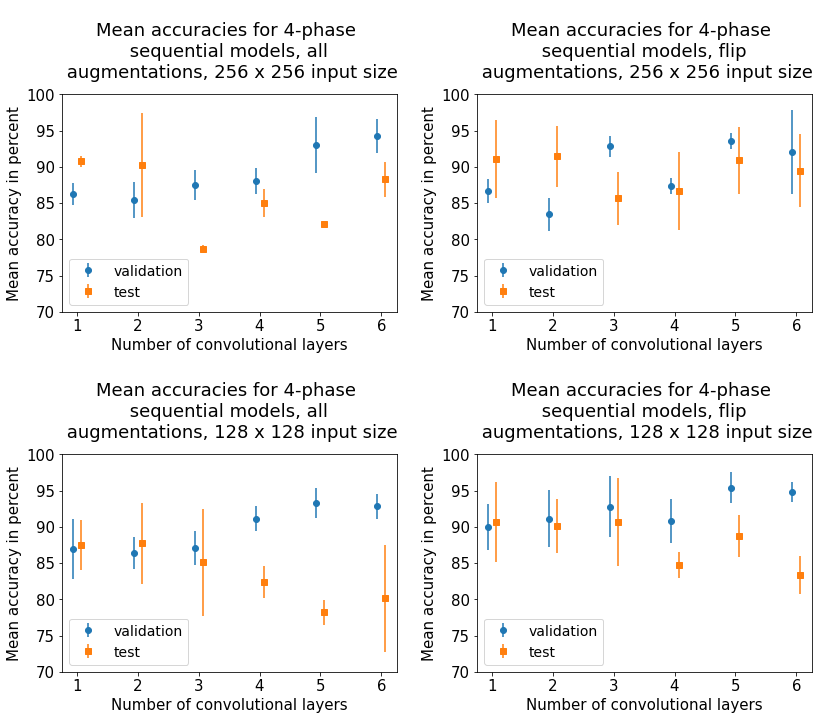
\includegraphics[width=6.6in]{images/4-phase_graphs.png}
    \caption{Plots of the mean accuracies against number of convolutional layers for the 4-phase models over three training runs.}
\end{figure} 
%general increase in accuracy for validation vs decrease for test
%suggests overfitting with higher numbers of layers
%divergence of test and validation accuracy in all models except 256 flip
%flip augmentation better than all
%similar performance between both input sizes
%relatively small error bars on validation suggests good model stability
%need more trial runs for better picture of accuracy
%high overall accuracies show viability
%best test set accuracy, flip 256 2 layers
%isotropic always predicted correctly, possible leakage giving false indication of high %accuracy
%using flip 256 for other models
From the plots, we see that in general the validation accuracy has a slight positive correlation with the number of layers, with the opposite for the test accuracy. This trend is not so clear for the case of flip augmentations with $256 \times 256$ input size. The decrease in test set accuracy with higher numbers of layers is suggestive of overfitting, which is to be expected as the model capacity increases greatly with each added convolutional layer. The lower capacity models from this selection are, therefore, a better choice. The high validation accuracies at greater layer counts is potentially because of the fact that the models are saved at the point of highest validation accuracy during training, which can fluctuate to high numbers. The difference between some of the validation and test accuracies could also be due to the imbalance between the number of samples in each set, with almost double the number of validation samples as test.

In every case, for the same input size and number of layers, models with flip augmentations have a higher mean test set accuracy than with all augmentations. This suggests that some of the images produced by the extra augmentations are dissimilar to actual texture images. When applying the rotation, scaling, and translation transformations included in all augmentations, certain edges and corners of the image are extended or distorted to fill the input space. These regions do not contain features identifiable as liquid crystal texture, which could be the cause of the lower performance. In addition, the models with all augmentations took approximately twice as long to train as with flip augmentations, due to the increased computing time in applying the extra transformations.

With the same augmentations and number of layers, models with an input size of $256 \times 256$ performed better on the test set than $128 \times 128$, 10 out of 12 times. Certain textural features could have potentially been lost at the lower resolution, which could explain the lower accuracies observed. In addition, there was no significant reduction in model training time with the $128 \times 128$ input size, despite smaller convolution operations and GPU memory requirements.

Overall, the models achieved good accuracies on the test set, with 10 out 24 scoring above 90 percent. This demonstrates the viability of CNNs in the liquid crystal phase identification task. However, the textures of the four phases these models were trained to classify are highly distinct and potentially easily identified by the human eye, meaning even the best models would perhaps not be useful at this stage. The most straightforward way to improve the results would be through increasing the size of the dataset, and adjusting model capacity appropriately.

The highest accuracy on the test set out of every trained model was 94.33 percent. This was one of the models with two convolutional layers, flip augmentations, and $256 \times 256$ input size. The lowest had 74.42 percent accuracy, with 6 convolutional layers, all augmentations, and $128 \times 128$ input size. Figure 4 displays the test set confusion matrices for these models.
\begin{figure}[!htb]
	\centering
    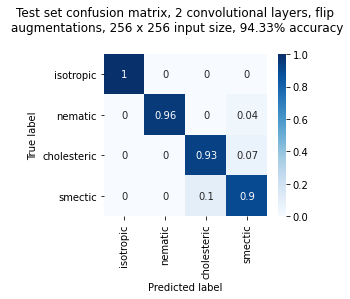
\includegraphics[width=6in]{images/confusion_matrix.png}
    \caption{Test set confusion matrices for the models with highest and lowest overall test accuracies. The value in each square represents the fraction of examples with the true phase label for which the model output was the predicted phase label. We therefore aim for values close to one along the diagonal, which corresponds to correct model outputs.}
\end{figure} 
We see that both models, especially the less accurate one, perform the worst on the cholesteric and smectic phases, suggesting that they have a higher degree of similarity between their textural features than the other classes. Both models identify the nematic phase more than 95 percent of the time, and are completely accurate in identifying the isotropic phase and do not miss-label any other phases as isotropic. This high isotropic  success rate is potentially a result of the uniformity of the generated dark isotropic textures, which do not have highly complex features for the model to learn. Upon removal of the isotropic class from the test set, the most accurate model's accuracy is reduced to 92.57 percent, and the least accurate to 66.86. The isotropic class could, therefore, be viewed as a source of data leakage for these models. However, it does suggest that the models would easily be trained to identify real isotropic textures. 
%=========================================================================================
\subsection{Models II, smectic A and C binary classifiers}
\subsubsection{Dataset construction II}
The next set of models were an attempt at the binary classification task of smectic A and C phases, which can have similar textural features due to their structures only differing by a tilt in the director \cite{Dierking03}. The distribution of data for the two classes is displayed in Table 2.
\begin{table}[!htb]
\begin{center}
\caption{Dataset distribution for smectic A and C classifier models.}
\begin{tabular}{l|c|c|c|c}
\toprule
& \textbf{SmA} & \textbf{SmC} & \textbf{Totals} & \textbf{\% of total}\\
\midrule
\textbf{Training} & 719 & 1067 & 1786 & 70.17\\
\textbf{Validation} & 174 & 183 & 357 & 14.03\\
\textbf{Test} & 204 & 198 & 402 & 15.80\\
\midrule
\textbf{Totals} & 1097 & 1448 & 2545\\
\bottomrule
\end{tabular}
\end{center}
\end{table}
The validation and test sets are more equally balanced for this set of models. All polarised microscopy videos used in this set were provided by project supervisor Ingo Dierking, and all images were again prepared as in Section 3.2.2.
\subsubsection{Model architectures and training configuration II}
Based on the results of Section 3.3, flip augmentations and an input size of $256 \times 256$ were used for all smectic A and C models. The binary cross-entropy loss function is used, with one output unit for every model. The same six sequential model configurations as for the 4-phase classification task were tested, with reduced numbers of hidden units to prevent overfitting because the dataset is smaller. In this case, the final convolutional layer for each sequential model has 32 channels, with the number of channels halving with each convolutional layer going backwards through the model. Therefore, the six convolutional layer model has only one channel in its first layer. The number of hidden units in the dense layers is also reduced, with 32 in the first and 16 in the second for all sequential models.

A different type of CNN architecture was also tested for smectic A and C, inspired by Google's 22 layer GoogLeNet Inception model, the winner of the ILSVRC in 2014 \cite{ILSVRC15}. An Inception model contains branching "Inception blocks", a specific arrangement of convolutional layers depicted in Figure 5 \cite{Szegedy2015}.  
\begin{figure}[!ht]
\centering
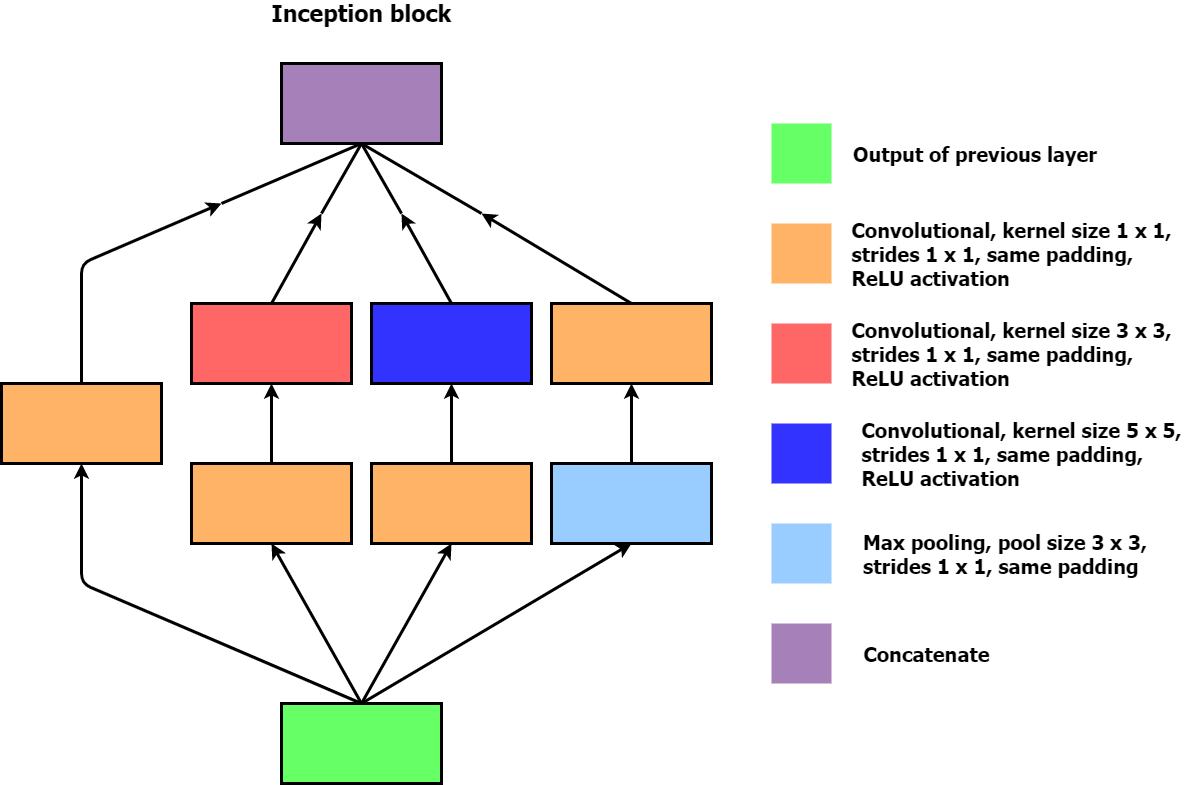
\includegraphics[width=5in]{images/inception_block.png}
\caption{Architectural diagram of an Inception block. The input is shared between 4 parallel convolution operations, with their outputs being concatenated along the channel axis in the final layer. This results in the output having a number of channels equal to the sum of the number of channels of each concatenated layer. Different kernel sizes in each parallel layer can extract different sized features from the input, propagating more information through the output of the block. The $1 \times 1$ kernel layers preceeding the $3 \times 3$ and $5 \times 5$ ones can be used to reduce the number of channels and, therefore, the computational cost, if necessary. The pooling layer is there to provide some translational invariance \cite{Szegedy2015}.}
\end{figure}
Three Inception models were used for smectic A and C, containing one, two and three Inception blocks. Similarly to GoogLeNet, each one starts with a convolutional layer with kernel size $7 \times 7$, 2 channels and same padding, followed by a standard pooling layer. This is followed by two more convolutional layers, first with kernel size $1 \times 1$, 4 channels and valid padding, and second with kernel size $3 \times 3$, 8 channels and same padding, before another standard pooling layer. This is proceeded by the Inception blocks. The number of channels in each layer in a block is reduced by the $1 \times 1$ kernel layers, and starts at 8 for the first, doubling with each successive block. The final inception block is followed by average pooling with pool size and strides of $5 \times 5$ and valid padding. This is followed by a convolutional layer with kernel size $3 \times 3$, a number of channels equal to half that of the output of the final inception block, and same padding. Similarly to the sequential models, it is finished with global average pooling, followed by two dense layers, first with a number of hidden units equal to the channels in the previous convolutional layer, and second with half that number, before the final single output unit. As an example, the architecture of the inception model with one block is outlined in Figure 9 in Appendix C.
\subsubsection{Results II}
Similarly to the 4-phase models, all sequential and Inception smectic A and C models were trained three times and the mean validation and test accuracies calculated, with an uncertainty of half the range. These results are shown in Figure 6. 
\begin{figure}[!ht]
	\centering
    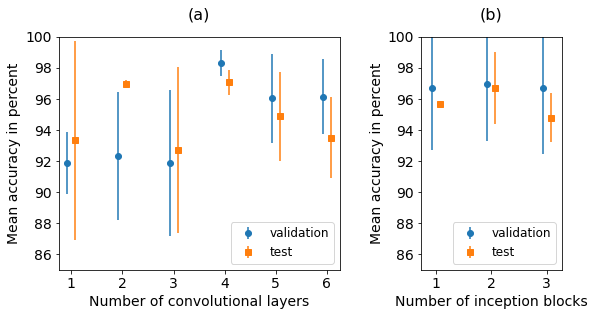
\includegraphics[width=5.6678in]{images/smecticAC_graphs.png}
    \caption{Plots of the mean accuracies over three training runs against number of convolutional layers for sequential models, and number of Inception blocks for Inception models, for the smectic A and C models.}
\end{figure} 
%no noticeable trends in accuracies for either type
%overall very good accuracies
%large error bars, need more trial runs
%overall inception better than sequential
We do not observe any noticeable trends in either validation or test accuracy, and most of the models have similar scores on both sets.

All nine models achieved a mean test accuracy above 90 percent, with four above 95. This is a strong performance, demonstrating the viability of CNNs in differentiating similar-looking liquid crystal textures. However, it is a simple binary classification problem, so larger datasets with more phases will be required to test the limits of these types of models. The Inception models have a greater minimum mean test accuracy than the sequential ones, with 94.79 percent compared to 92.71. However, the highest mean test accuracy of 97.05 percent belongs to the sequential model with four convolutional layers. More training will have to be carried out to draw confident conclusions about the architecture that performs better overall.

The error bars are very large on some of the data points, suggesting that certain models in this task are highly sensitive to the stochastic properties of training. The error could be reduced to provide a more confident estimation of each model's overall accuracy by increasing the dataset size and performing more training runs. A single training cycle takes a long time, approximately one hour, with the set up used to train these models, which is the limiting factor in producing more results and higher accuracies. Larger models with bigger datasets will also take longer to train.

The single saved model with the highest test accuracy at 99.22 percent was an Inception model with two blocks, and the lowest was a sequential model with one convolutional layer, at 85.42 percent. The confusion matrices for these models are displayed in Figure 7.
\begin{figure}[!ht]
	\centering
    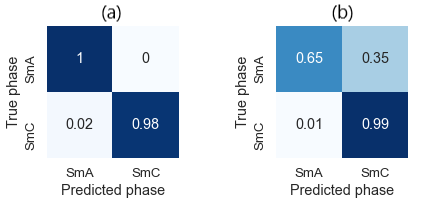
\includegraphics[width=4.174in]{images/confusion_matrix_2.png}
    \caption{Test set confusion matrices for the smectic A and C models with highest and lowest overall test accuracies.}
\end{figure} 
The Inception model misidentifies two percent, or four samples, of the smectic C test images. This is likely a fluctuation and may not represent the model's true generalisation error, due to the relatively small size of the dataset. The sequential model's inaccuracies mostly stem from misidentifying smectic A as smectic C, which is potentially due to there being more smectic C samples than A in the training set. 
%=========================================================================================
\subsection{Models III, general smectic classifiers}
\subsubsection{Dataset construction III}
Exactly the same models, aside from the number of output units, as the smectic A and C classifiers were tested in the identification of the fluid smectic, hexatic smectic, and soft crystal phases. The dataset distribution is presented in Table 3.
\begin{table}[!htb]
\begin{center}
\caption{Dataset distribution for general smectic classifier models.}
\begin{tabular}{l|c|c|c|c|c}
\toprule
& \textbf{FSm} & \textbf{HSm} & \textbf{SC} & \textbf{Totals} & \textbf{\% of total}\\
\midrule
\textbf{Training} & 1759 & 486 & 600 & 2845 & 70.67\\
\textbf{Validation} & 372 & 90 & 144 & 606 & 15.05\\
\textbf{Test} & 389 & 90 & 96 & 575 & 14.28\\
\midrule
\textbf{Totals} & 2520 & 666 & 840 & 4026\\
\bottomrule
\end{tabular}
\end{center}
\end{table}
Again, all videos used in this set were provided by project supervisor Ingo Dierking, and all images for this set were prepared as in Section 3.2.2. The current collection of polarised microscopy videos gives an image dataset that is greatly imbalanced in favour of the fluid smectic phases. 
\subsubsection{Model architectures and training configuration III}
The nine models used for the general smectic phase classification have the same architectures and training configurations as those of section 3.4.2, aside from using the categorical cross-entropy loss instead of binary cross-entropy and having three final layer output units instead of one. 
\subsubsection{Results III}
When training the sequential models on the dataset, despite some trial and error adjustments to the sizes of the hidden layers, every model predicted fluid smectic 100 percent of the time on the test set. This is most likely due to the large imbalance in the dataset. The sequential models are possibly unable to learn enough features from the small sets of hexatic smectic and soft crystal data, collapsing into predictions of fluid smectic every time, which results in an accuracy on the test set of 67.65 percent. This is simply equal to the percentage of fluid smectic examples in the test set.

The Inception models were trained on this set one time each, with some more successful results. The test set accuracies were 72.24, 83.27, and 85.48 percent for one, two and three blocks respectively. The models are still biased towards the fluid smectic class. However, they can identify the other phases, for example the three-block model correctly classifies 62 percent of the hexatic smectic and 83 percent of the soft crystal phases. The Inception models' performance is potentially better than that of the sequential models due to the range of different kernel sizes, which are able to extract features of varying size. More data, especially for the hexatic smectic and soft crystal phases, will be needed to conduct a more concrete investigation.
%=========================================================================================
\section{Conclusions}
%first half of project set out to establish wether or not machine learning can be used to classify small numbers of basic liquid crystal phases
%more time needed to perform reruns to reduce error and test different architectures
%data limiting factor, need more to improve models and create models that classify more phases
%from 4-phase, conclude that 256 input and flip augs is good setting
%overall, promising results with high accuries displayed
In this beginning half of the project, we have endeavoured to establish a well-formed liquid crystal texture dataset, and investigate the viability of machine learning algorithms in identifying the different liquid crystal phases from the dataset. The approach so far has considered deep convolutional neural networks, in three separate phase classification tasks. 

From the 4-phase model investigations, we draw the conclusion that the flip augmentations are less computationally expensive and time consuming to use, and produce more accurate models than using the all augmentations setting. Also, when comparing the two input sizes of $256 \times 256$ and $128 \times 128$, the former results in higher accuracies with no increase in model training time. In general, the 4-phase models perform well on the test set, showing that CNNs have the potential to be an effective choice of machine learning algorithm type.

The extremely high performance of the smectic A and C binary classifier models further demonstrates the efficacy of CNNs in identifying liquid crystal phases, including ones with fewer distinguishable textural features. The Inception and sequential models both achieve good results. The large deviations in accuracy on repeated training runs of these models shows that final model accuracy can vary greatly, depending on the parameter initialisation values and the randomly selected and augmented training data minibatches. Increased confidence in average accuracy requires further training runs, which is limited by long training times. 

Despite having built a substantial overall collection of texture images, the general smectic phase model investigation highlights the requirement for balanced classes and a large training set in order for models to generalise well. A lack of data in the hexatic smectic and soft crystal phases results in poor performance, with the sequential models outputting a fluid smectic prediction for every input. The Inception models offer a marginal improvement in this case, however the accuracies on the test set are still lower than would be required of a reliable model.
%=========================================================================================
\section{Going forward}
%different architectures
%models classifying more phases
%colour image investigations
%physical property investigations
%more data
For the second half of this project, there are a variety of potential ways to expand upon the current work and take it in different directions. Other types of CNNs with branching architectures could be investigated, as well as larger models trained with more data that can classify a greater number of liquid crystal phases. Entirely different deep learning algorithms could also be investigated, transformer networks in particular. The usage of coloured image inputs could be tested, to determine whether or not this would lead to better generalisation or simply create data leakage. If the data and labels become available, regression models for physical properties of liquid crystals such as cholesteric pitch length could be investigated.
%=========================================================================================

\bibliography{report}

\appendix
\appendixpage
\section{Training algorithms}
\subsection{Backpropagation}
For a fully connected feedforward neural network, the backpropagation algorithm is used to compute the gradient of the cost function with respect to all trainable parameters, $\bm{g}=\bm\nabla_{\bm\theta}J$. $\bm{g}$ is composed of the gradients of $J$ with respect to the weights and bias parameters for each layer $l$, $\bm\nabla_{\bm{w}_l}J$ and $\bm\nabla_{\bm{b}_l}J$. Let us define $\bm{\mathcal{G}}$, a vector with variable size that is updated with the gradient of each layer as we move backwards through the network. At the start of backpropagation, we assign the gradient on the final layer outputs to $\bm{\mathcal{G}}$,
\begin{equation}
\bm{\mathcal{G}}\leftarrow \bm\nabla_{\bm{O}_D}J=\bm\nabla_{\hat{\bm{y}}}J, 
\end{equation} 
obtained from the derivative of the loss function $L(\hat{\bm{y}},\bm{y})$ with respect to $\hat{\bm{y}}$. We then perform $D$ steps with layer number $l$ decreasing by one each time. For each step, we first update $\bm{\mathcal{G}}$ by changing it from a gradient on the layer's output to a gradient on the non-activated output, by the chain rule,
\begin{equation}
\bm{\mathcal{G}}\leftarrow \bm{\nabla}_{\bm{h}_l}J=\bm{\mathcal{G}}\odot A'(\bm{h}_l).
\end{equation}
The parameter gradients for the layer are given at this point by
\begin{align}
\bm\nabla_{\bm{w}_l}J&=\bm{\mathcal{G}}\bm{O}_{(l-1)}^{\top},\\
\bm\nabla_{\bm{b}_l}J&=\bm{\mathcal{G}}.
\end{align}
To finish the step, the gradient is propagated onto the output of the next lower hidden layer,
\begin{equation}
\bm{\mathcal{G}}\leftarrow \bm{\nabla}_{\bm{O}_{(l-1)}}J=\bm{w}_l^{\top}\bm{\mathcal{G}}.
\end{equation}
Upon reaching $l=1$, all parameter gradients have been obtained and the algorithm is complete \cite{Rumelhart86, Goodfellow16}.

\subsection{Adam optimiser}
The Adam stochastic optimiser algorithm proceeds as follows. Before the first iteration, the biased gradient first and second moment estimate variables, $\bm{s}$ and $\bm{r}$, and the timestep, $t$, are initialised to zero. At the start of each iteration, a minibatch of data is sampled and $\hat{\bm{g}}$ is calculated as in Equation 13. $t$ is updated as
\begin{equation}
t\leftarrow t+1,
\end{equation}
$\bm{s}$ is updated as
\begin{equation}
\bm{s}\leftarrow \beta_1\bm{s}+(1-\beta_1)\hat{\bm{g}},
\end{equation}
and $\bm{r}$ is updated as
\begin{equation}
\bm{r}\leftarrow \beta_2\bm{r}+(1-\beta_2)\hat{\bm{g}}\odot\hat{\bm{g}},
\end{equation}
where $\beta_1$ and $\beta_2$ are the first and second moment exponential decay hyperparameters. The bias-corrected first and second moments, $\hat{\bm{s}}$ and $\hat{\bm{r}}$, are then updated as
\begin{equation}
\hat{\bm{s}}\leftarrow \frac{\bm{s}}{1-\beta_1^t},
\end{equation}    
and
\begin{equation}
\hat{\bm{r}}\leftarrow \frac{\bm{r}}{1-\beta_2^t}.
\end{equation}
In the final step of the iteration, the parameters of the model are updated as
\begin{equation}
\bm{\theta}\leftarrow \bm{\theta}-\alpha\frac{\hat{\bm{s}}}{\sqrt{\hat{\bm{r}}}+\epsilon},
\end{equation}
where $\alpha$ is the step size hyperparameter and $\epsilon$ is a small hyperparameter for numerical stability. Iterations are carried out until model training is complete. The recommended defaults for the hyperparameters are $\alpha=0.001$, $\beta_1=0.9$, $\beta_2=0.999$ and $\epsilon=10^{-8}$ \cite{Kingma14}.     

\section{Example architecture diagrams}
Figure 8 provides a representation of the network architecture of the 4-phase sequential model with three convolutional layers and $256 \times 256$ input size.
\begin{figure}[!htb]
\centering
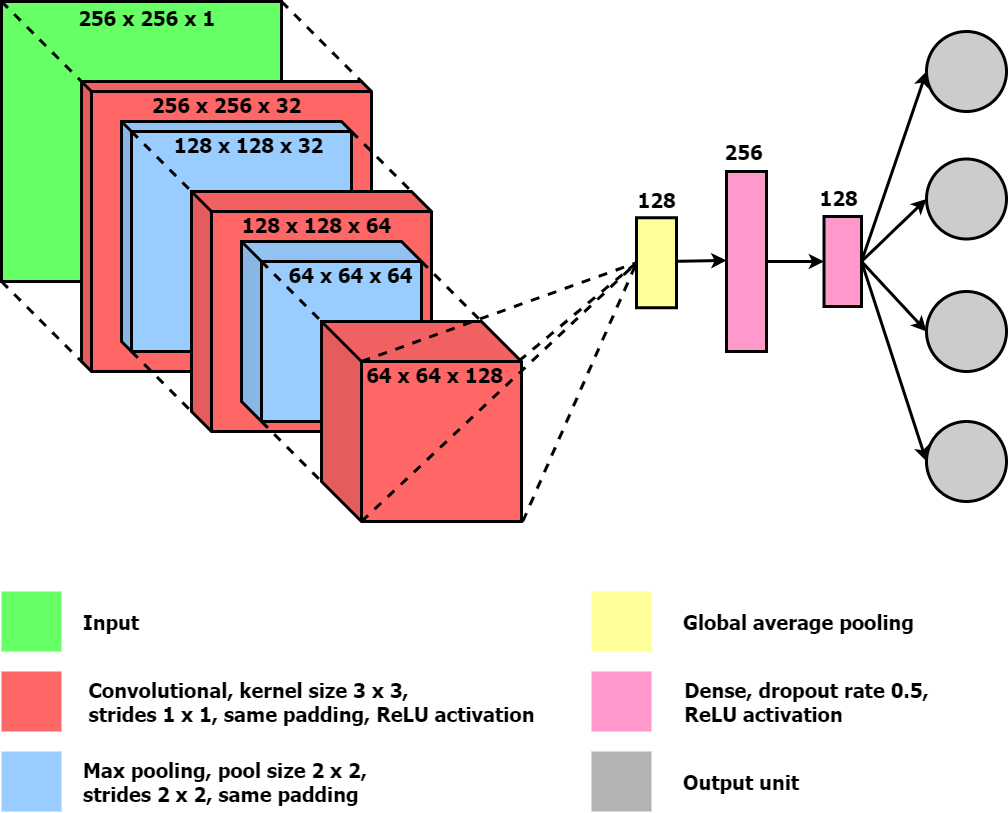
\includegraphics[width=5.5812in]{images/v3_conv_3_diagram.png}
\caption{Architectural diagram of the sequential CNN model with input size $256 \times 256$ and three convolutional layers. The output dimensions are displayed as width $\times$ height $\times$ channels for each convolutional and max pooling layer. Not to scale.}
\end{figure}
Figure 9 provides a representation of the network architecture of the smectic A and C Inception model with one block.
\begin{figure}[!htb]
	\centering
    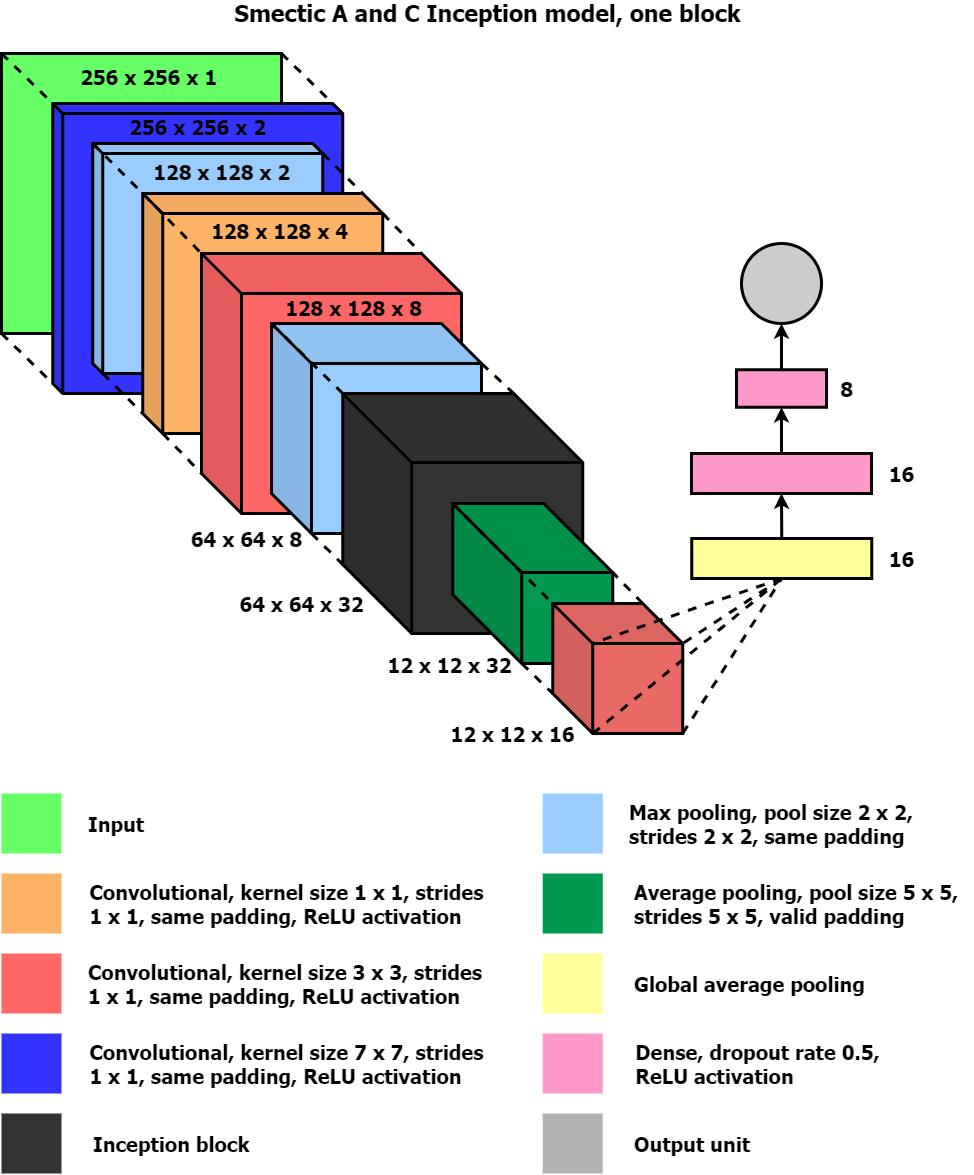
\includegraphics[width=5.393in]{images/inception_model.png}
    \caption{Architectural diagram of the Inception CNN model with one block. The output dimensions are displayed as width $\times$ height $\times$ channels for each convolutional, max pooling and Inception block layer. Not to scale.}
\end{figure} 
\end{document}